
\chapter{Testing and simulation}
\label{testing}

% Description of what tests has been performed.


\section{Simulation}

This Petri net model, simulation and analysis project has been inspired by the author's current work in the Generic Distributed Exact Cover Solver (DECS) \cite{decs-web} project.
DECS details the implementation of a distributed computing system to solve exact cover problems by using Donald Knuth's Dancing Links (DLX) \cite{knuth00dancing} algorithm.
Figure \ref{fig:architecture} provides the basic architecture of this distributed computing system.

DECS mainly works by dividing a problem into smaller pieces and through distributed computing middleware it distributes these pieces to a collection of client systems.
It uses a system called BOINC \cite{boinc} to handle the work distribution and result collection process.
In BOINC the clients send HTTP GET and PUT messages to a web server in order to download more work and upload the results.


\subsection{Model}

The Petri net model is based on the architecture as shown in Figure \ref{fig:architecture}.
In order for the simulation to be useful the complete request/response cycle needs to be modeled.
The firing times of the transitions will also have to be determined by research and testing.


\subsubsection{Assumptions}

To begin with we have to make a few assumptions regarding the system we are trying to model.
We do this in order to make the model simple and easy to understand.
Because we are dealing with a distributed system we need to be aware of the most common pitfalls we might encounter.
From ``The eight fallacies of distributed computing'' \cite{distributed-fallacies} the following assumptions apply to our model:

\begin{itemize}
	\item The network is reliable.
	\item Topology does not change.
\end{itemize}

We assume that all the hardware and the software in the distributed system is reliable.
Without this assumption we would have to take into account all sorts of failure scenarios.
The model also assumes that the network topology does not change significantly.
BOINC itself can deal with several different changes to topology, like disconnected clients and wireless roaming clients, etc., but to make the model simple we assume that the clients are always reachable through the network.

However, there are some of the eight fallacies we do NOT make assumptions about or which do not apply to this project:

\begin{itemize}
	\item Latency is zero.
	\item Bandwidth is infinite.
	\item The network is secure.
	\item There is one administrator.
	\item Transport cost is zero.
	\item The network is homogeneous.
\end{itemize}

Zero latency is not assumed because the latency of the distributed system is modeled by the firing time of each of the transitions.
In the cases where it counts we do not assume infinite bandwidth.
However, it is difficult to accurately model both the bandwidth limitation and the latency between the clients and the server without making the model significantly harder to understand.
The current solution is a compromise between accuracy and readability.
BOINC handles all the network communication and carries the burden of securing the distributed system against attacks.
We do not model these security mechanism because they have no direct impact on the performance of the system.
The ``one administrator'' and ``zero transport cost'' assumptions fall outside the scope of this report.
Put more plainly: We do not care how this system is administered and how much the infrastructure costs would be.
As far as BOINC goes it does not care what platform the server or clients run because it is able to supports most major operating systems and hardware platforms.
Some additional assumptions are presented later under the sections they belong to.


\subsubsection{Server model}

We begin by first modeling the server in this distributed computing system.
We also make the assumption that there is only one server, even though BOINC can support more than one.
The server has two ``pipelines'' so to speak: The request pipeline and the response pipeline.
In Figure \ref{fig:server} you can see the complete server model.

\begin{figure}[htbp]
	\centering 
	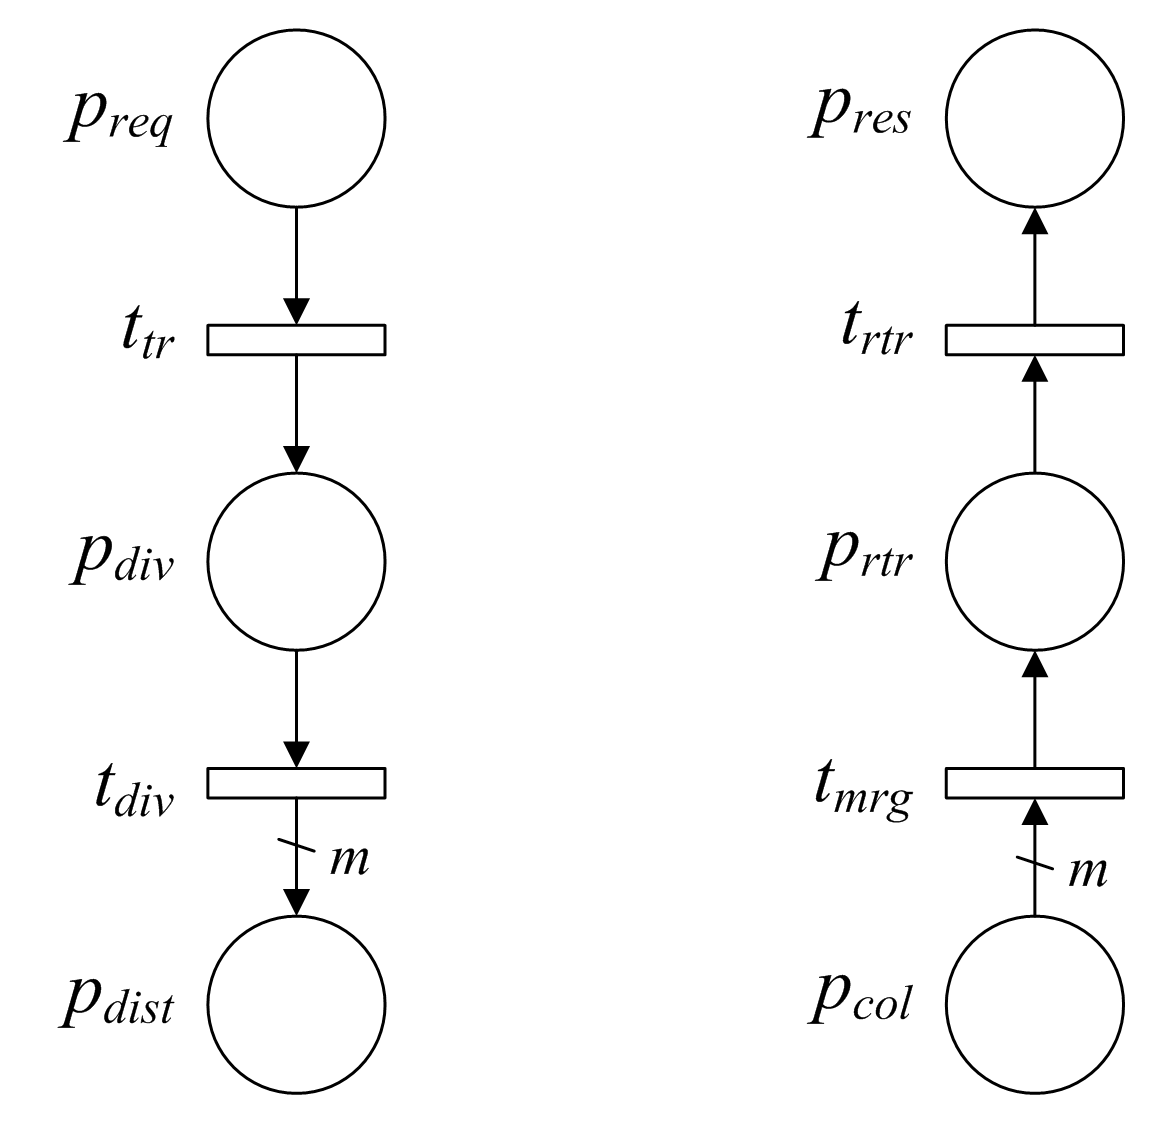
\includegraphics[width=0.6\textwidth]{server.png}
	\caption{Petri net module for the distributed computing server}
	\label{fig:server}
\end{figure}

The request pipeline begins with the place $p_{req}$ onto which an application may place a specific exact cover problem to be processed by the distributed computing system.
The specific problem is then transformed into a more generic form by the transition $t_{tr}$ before it is placed in $p_{div}$.
From there the problem is divided into several smaller problems by $t_{div}$ and the resulting pieces\footnote{BOINC uses the term ``work units'' instead of pieces, but it is essentially the same thing.} are placed in $p_{dist}$ to be distributed to the clients.
The weight, $m$, of the arc from $t_{div}$ to $p_{dist}$ is the number of pieces the problem is divided into.

The response pipeline starts with the place $p_{col}$ where the solutions from the clients are placed.
When all the solutions have arrived they are merged together by $t_{mrg}$ and the resulting solution is placed in $p_{rtr}$.
The weight of the arc from $p_{col}$ to $t_{mrg}$ will also have to be $m$ in order to ensure that the merging process does not take place before all the solutions has arrived.
From $p_{rtr}$ the generic solution is transformed back into the domain of the specific problem by $t_{rtr}$ and returned to the application in $p_{res}$.


\subsubsection{Client model}

\begin{figure}[htbp]
	\centering 
	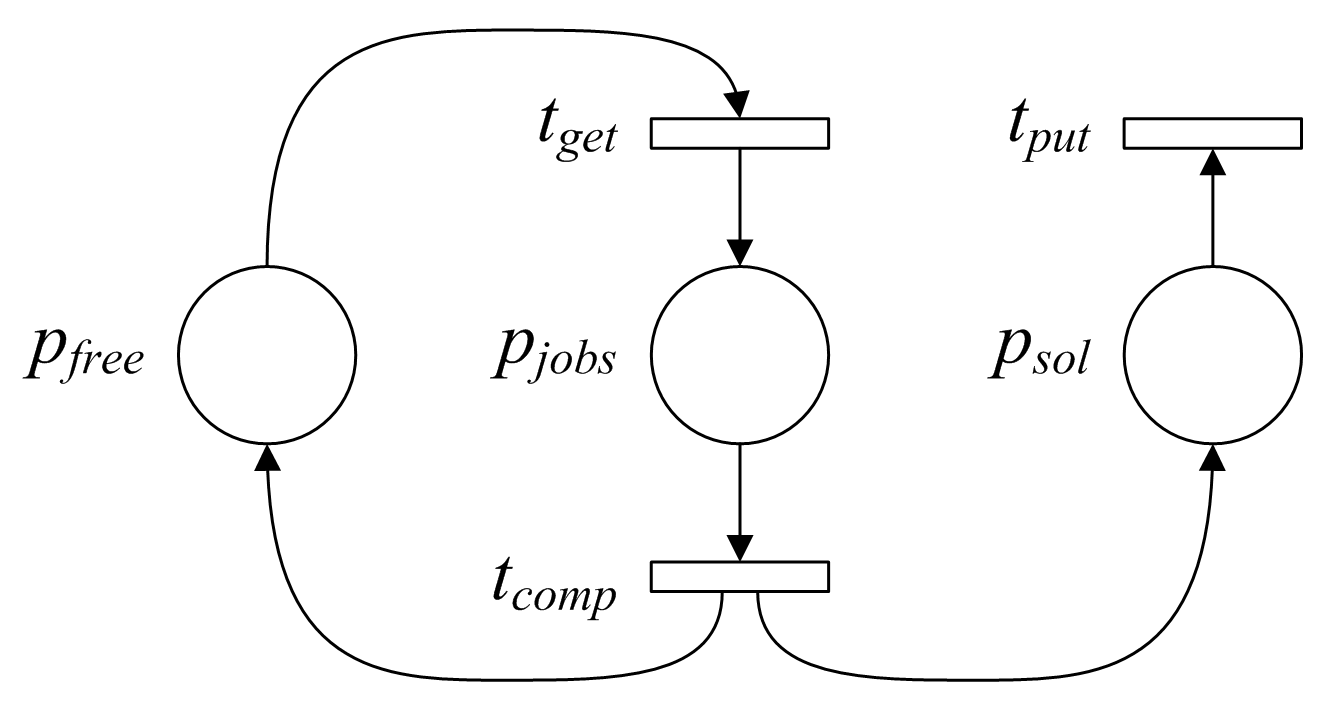
\includegraphics[width=0.8\textwidth]{client.png}
	\caption{Petri net module for the distributed computing clients}
	\label{fig:client}
\end{figure}

Figure \ref{fig:client} shows the Petri net of the compute clients.
To identify each client they are given a number $i$ from $1$ to $n$.
When $t_{get,i}$ is fired the HTTP GET request is send to the server and a piece of the problem is returned to the client and placed in $p_{jobs,i}$, which is a job queue.
$t_{comp,i}$ is the computing program which processes each job from $p_{jobs,i}$ one at a time.
This model assumes that the computing program is only able to process one problem at the same time, even on multi-processor systems.
When a computation is complete the resulting solution is placed in $p_{sol,i}$ and then sent to the server by $t_{put,i}$.
$p_{free,i}$ is used to control the number of simultaneous pieces that a client can work on at the same time.


\subsubsection{Network model}

\begin{figure}[htbp]
	\centering 
	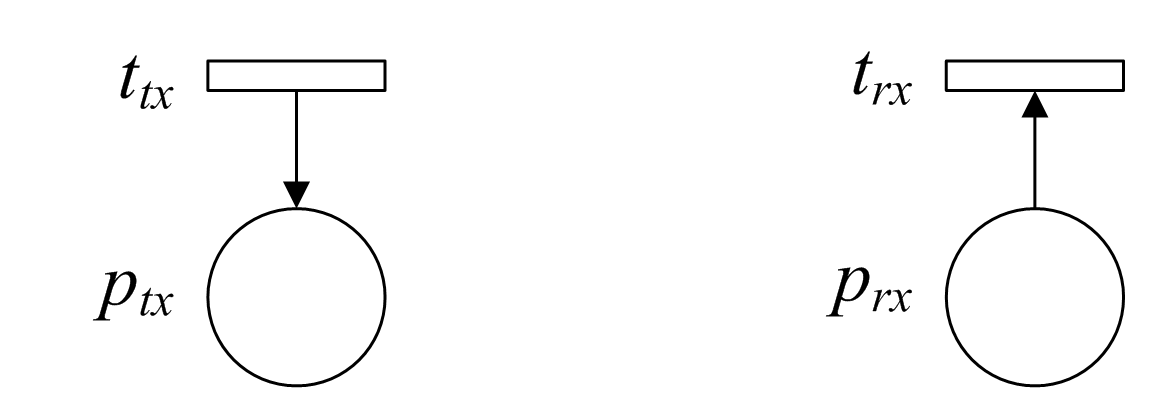
\includegraphics[width=0.6\textwidth]{network.png}
	\caption{Petri net module for the distributed computing network}
	\label{fig:network}
\end{figure}

In an attempt to model the bandwidth limitation on the server side the Petri net in Figure \ref{fig:network} has been designed.
It is a primitive bandwidth throttling device and with the correct firing times it should be able to regulate the flow of data coming from and going to the server.
$t_{tx}$ and $p_{tx}$ model the transmit limit and $t_{rx}$ and $p_{rx}$ model the receive limit.
It is assumed that the network communication channel is full duplex\footnote{Full duplex allows data to be sent and received at the same time.} and that the combined network bandwidth of all the connected clients is equal to or larger than the bandwidth on the server side.
This means that we are assuming that the bottleneck is on the server side, which is true in most cases where the number of clients is high.
Modeling the individual bandwidth limitation for each client and the overhead of the TCP/IP and HTTP protocols themselves would result in an overly complex model.


\subsubsection{Petri net definition}

A Petri net graph is a weighted bipartite graph $(P, T, A, w)$.
$P$ is the set of places, $T$ is the set of transitions, $A$ is the set of arcs and $w$ is the arc weight function.
A complete system with one client will look like Figure \ref{fig:system}.
If additional clients are added the complexity steadily increases.
Below we have defined the complete Petri net model as shown in the figure.

\begin{align*} 
P &= \left\{p_{req}, p_{res}, p_{rtr}, p_{div}, p_{dist}, p_{col}, p_{tx}, p_{rx}, p_{free}, p_{jobs}, p_{sol}\right\} \\
T &= \left\{t_{tr}, t_{rtr}, t_{div}, t_{mrg}, t_{tx}, t_{rx}, t_{get}, t_{comp}, t_{put}\right\} \\
A &= \{(p_{req}, t_{tr}), (t_{tr}, p_{div}), (p_{div}, t_{div}), (t_{div}, p_{dist}), (p_{col}, t_{mrg}), (t_{mrg}, p_{rtr}), \\
&(p_{rtr}, t_{rtr}), (t_{rtr}, p_{res}), (p_{dist}, t_{tx}), (t_{rx}, p_{col}), (p_{tx}, t_{get}), (t_{put}, p_{rx}), \\
&(t_{get}, p_{jobs}), (p_{jobs}, t_{comp}), (t_{comp}, p_{free}), (p_{free}, t_{get}), (t_{comp}, p_{sol}), \\
&(p_{sol}, t_{put})\} \\
w&(t_{div}, p_{dist}) = m \\
w&(p_{col}, t_{mrg}) = m \\
\end{align*}

\begin{figure}[htbp]
	\centering 
	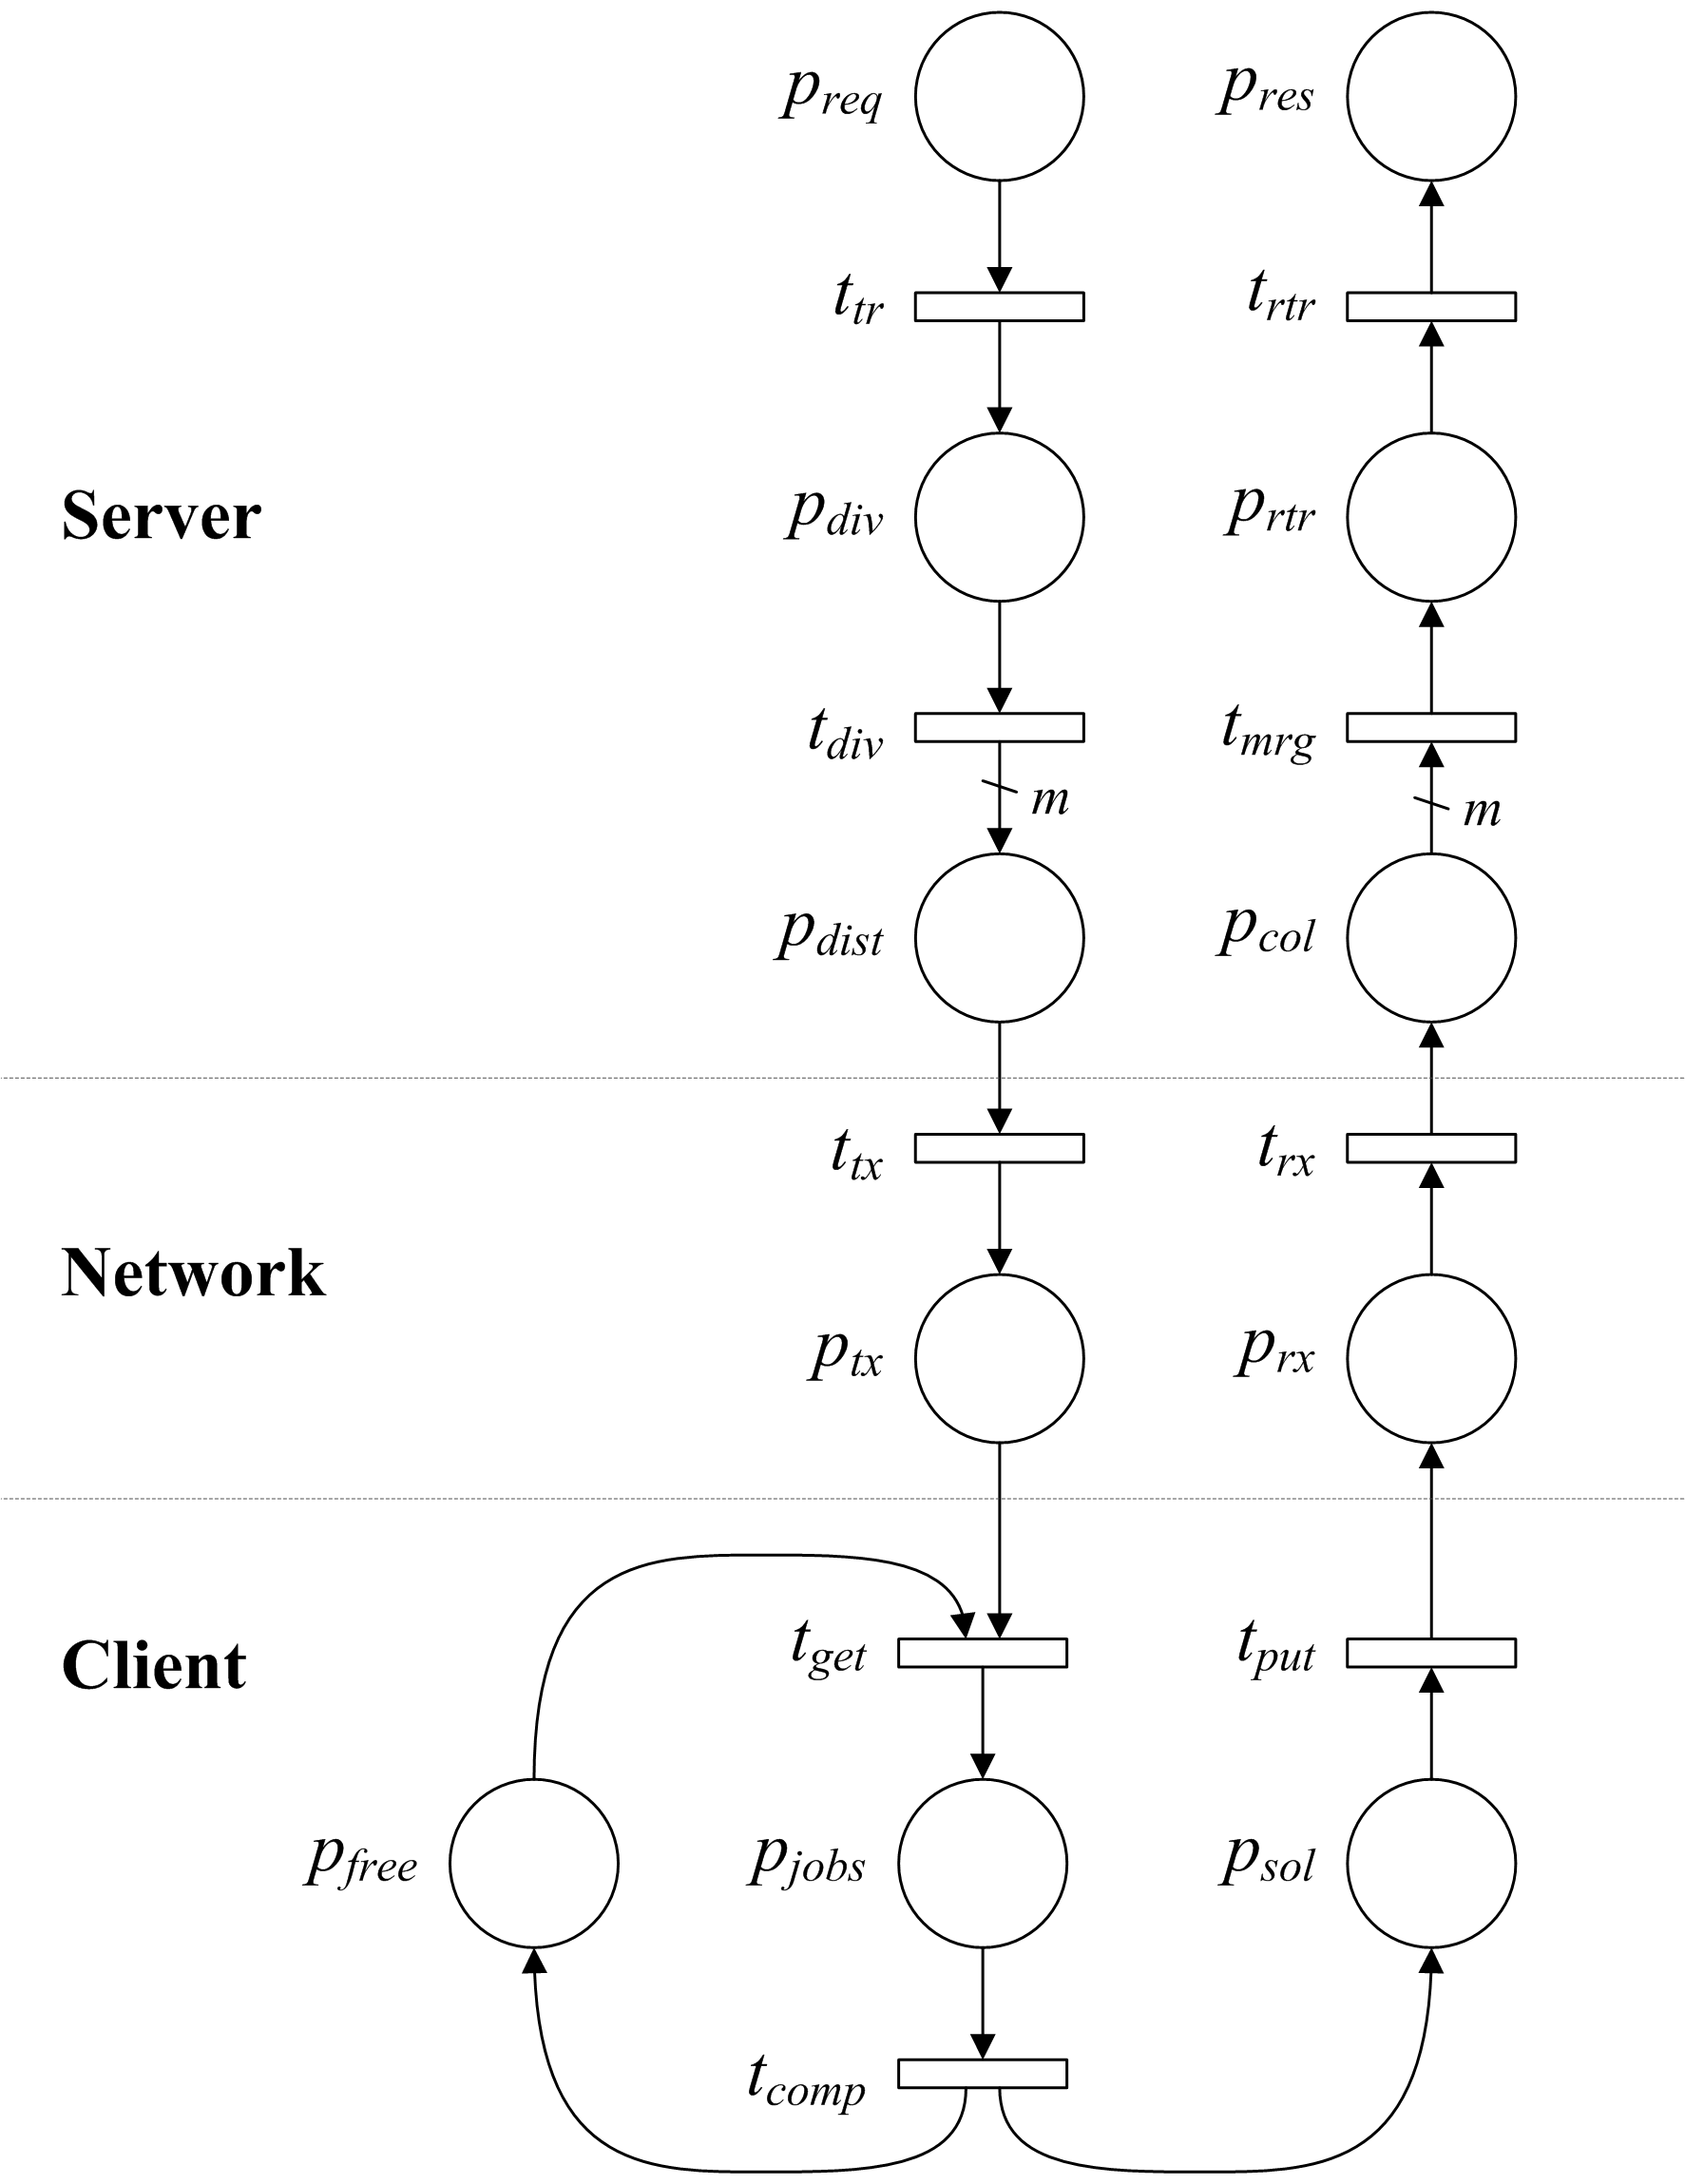
\includegraphics[width=1.0\textwidth]{system.png}
	\caption{A complete Petri net model for the distributed computing system}
	\label{fig:system}
\end{figure}


\subsection{Simulation}

We are going to use GPenSIM \cite{gpensim} version 2.1 to model and simulate the distributed computing system.
GPenSIM is a software package for MATLAB which enables you to use all the powerful facilities for statistics and plotting which MATLAB is known for.


\subsubsection{Simulation parameters}

To fully define the model a set of different parameters has to be defined.
These parameters are the firing times of the transitions, arc weights, number of clients and the initial dynamics\footnote{The initial dynamics/markings is the number and location of tokens at the start of the simulation.}.

To be able to find the correct parameters we need to specify what problem we want DECS to solve.
Lets say that we want to solve the 20-queens problem.
It should take about 12 hours of CPU time to solve this problem according to the NQueens@Home project \cite{nqueensathome}.
Although they use a specialized algorithm instead of the generalized DLX algorithm used in DECS, we assume that the running time is about the same.

For the number of clients we choose $n = 12$, meaning that if this was an ideal system the problem would be solved in 1 hour.
We want the clients to use around 10 minutes to solve each piece of the problem so we divide the problem into $m = 72$ pieces.
The transformation of the specific 20-queens problem to the DLX matrix takes 160 milliseconds so the firing time for $t_{tr}$ is 0.160 seconds.
The reverse transform, given that the number of solutions is about 39 billions, takes 39 seconds so that the firing time for $t_{rtr}$ is 39.
Dividing the problem into 72 pieces in DECS gives a firing time of 0.12 seconds for $t_{div}$.
Merging the solutions in $t_{mrg}$ results in a firing time of 7.2 seconds.
Since we model the solution of one problem we have to place one initial token in $p_{req}$.

Each of the problem pieces are 100 kilobit large and the server has a upstream bandwidth of 400 kbps (kilobit per second).
This will give us a throughput of 4 pieces per second which means that the firing time of $t_{tx}$ must be 0.25 second.
$p_{tx}$ should have a maximum number of tokens so that it better reflects the correct bandwidth when no more HTTP GET requests are being issued by the clients.
We choose to set this maximum limit to 4, which is the maximum number of pieces that can be send each second.
The downstream bandwidth of the server is 2000 kbps and each of the solutions has been compressed down to 8000 kilobit.
The rate of packets downstream will be 0.25 per second which results in a 4 second firing time of $t_{rx}$.

Each of the clients has an average round trip time (RTT) to the server of around 100 milliseconds.
For HTTP this gives a latency of $2*RTT +$ the time it takes to transfer the file.
The file transfer time has already been calculated so we ignore it in this case.
Since the RTT will usually vary a bit we use a normal distribution with a mean of 200 milliseconds and a standard deviation of 20 to generate random firing times for $t_{get}$ and $t_{put}$.
We set the firing time of $t_{comp}$ by using a uniform distribution with a minimum of 8 minutes and a maximum of 12.
We also put two tokens in $p_{free}$ to allow each client to retrieve two pieces of work from the server.


\subsection{Results}

From Figure \ref{fig:initdist} you can see that the primitive bandwidth throttling is doing its job.
It takes about 7 seconds to distribute the initial 24 pieces\footnote{Each of the 12 clients requests 2 pieces each to begin with because they have two tokens in $p_{free}$.} from $p_{dist}$ to the clients.

\begin{figure}[htbp]
	\centering 
	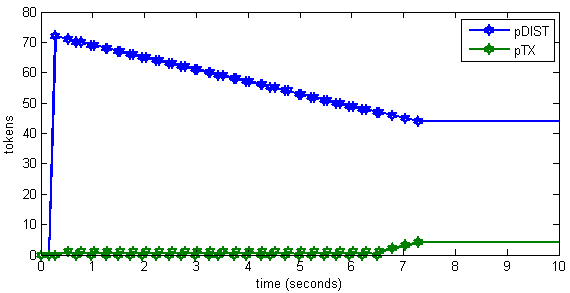
\includegraphics[width=1.0\textwidth]{initial_distribution.png}
	\caption{Initial distribution during the first 10 seconds}
	\label{fig:initdist}
\end{figure}

A complete simulation in GPenSIM takes 364 steps and depending on the random timing it finishes in about 67 minutes.
Figure \ref{fig:complete_sim} shows a complete simulation which only took 63 minutes.
You can clearly see the stages when each of the clients finish their work and request a new piece from the server.
Another simulation shown in Figure \ref{fig:complete_sim2} with the same parameters appears to have distributed the distribute and collect operations more evenly in time.
This would no doubt have caused less stress on the server and its bandwidth, but unfortunately it also hurts performance as it used 67 minutes in total to solve the problem.

\begin{figure}[htbp]
	\centering 
	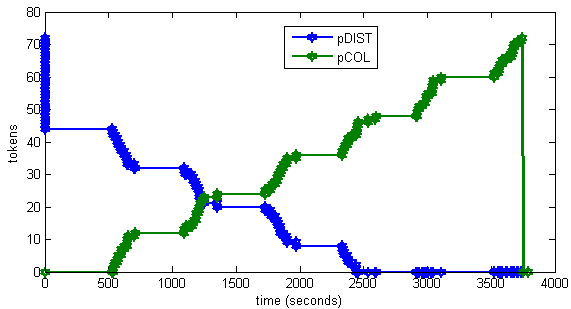
\includegraphics[width=1.0\textwidth]{complete_sim.png}
	\caption{Complete simulation of the distribution and collection completed in 63 minutes}
	\label{fig:complete_sim}
\end{figure}

\begin{figure}[htbp]
	\centering 
	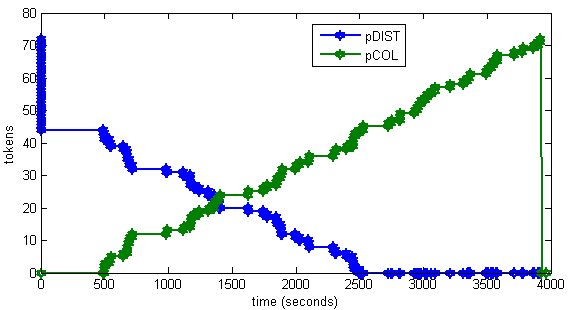
\includegraphics[width=1.0\textwidth]{complete_sim2.png}
	\caption{Another simulation of the distribution and collection completed in 67 minutes}
	\label{fig:complete_sim2}
\end{figure}


\subsection{Conclusion}

More accurate simulation results could probably be achieved by eliminating more of the assumptions and doing more research.
The main challenge in modeling this system was the distribution and collection mechanism and making sure that the latency and bandwidth limitations were preserved.
The model could be made more complex by incorporating other aspects of distributed computing as well.
Simulating client failure or malicious clients submitting incorrect data could be a possible extension.
That would require a certain piece of the problem to be sent to multiple clients for redundancy and verification.





\section{Performance}


